\subsection{二沉池}
\subsubsection{二沉池的选择}

普通辐流式二沉池的优点如下:
\begin{enumerate}
	\item 处理效率高:普通辐流式二沉池在处理污水时能够实现较高的沉降速度和较高的固液分离效率。通过合理的设计和操作,可以将污水中的悬浮颗粒和浮游生物有效地沉降到底部,从而实现高效的污水处理。
	\item 空间占用小:普通辐流式二沉池采用辐流式进出水方式,即进水和出水位于同一侧面,从而节省了空间。这对于一些空间受限的污水处理厂尤为重要,能够更好地满足设计要求。
	\item 操作维护简便:普通辐流式二沉池结构相对简单,没有复杂的机械设备或动力系统,因此操作和维护相对简单。这减少了运行成本和维护工作的复杂性,提高了处理厂的可靠性和稳定性。
	\item 适用性广泛:普通辐流式二沉池适用于各种规模的污水处理厂,无论是小型的社区处理厂还是大型的工业污水处理厂。它可以处理不同水质和污水特性的废水,具有较强的适应性和通用性。
	\item 抗负荷冲击能力强:普通辐流式二沉池在处理污水时具有较强的抗负荷冲击能力。它能够在短时间内应对污水负荷的变化,保持较高的处理效果,对于处理厂的稳定性和可靠性至关重要。
\end{enumerate}

综上所述,普通辐流式二沉池作为一种常用的污水处理工艺,具有高处理效率、小空间占用、简便的操作维护、广泛的适用性和强大的抗负荷冲击能力等优点。在设计污水处理厂时,选择普通辐流式二沉池是一个可靠和经济的选择,能够有效地处理污水并满足环境排放标准。


\subsubsection{计算数据与条件}

\begin{table}[H]
	\centering
	\caption{普通辐流式二沉池基础数据}
	\begin{tabular}{p{0.35\textwidth} *{3}{p{0.1\textwidth}}}
		\toprule
		参数    & 符号    & 值     & 单位 \\
		\midrule
		设计流量  & $Q$ & 35000 & m$^3$/d \\
		最大设计流量  & $Q_{max}$ & 58100 & m$^3$/d \\
		综合生活污水量变化系数 & $K_z$ & 1.66 &  \\
		\midrule
		氧化沟中悬浮固体浓度 & $X$    & 4000   & mg/L \\
		二沉池底流生物固体浓度 & $X_r$   & 10000   & mg/L \\
		污泥回流比 & $R$   & 100    & \% \\
		\bottomrule
	\end{tabular}%
	\label{tab:Basic data of ordinary radial secondary sedimentation tank}
\end{table}%

查阅刘振江和崔玉川主编的《城市污水厂处理设施设计计算》,得到普通辐流式沉淀池计算公式如下:

\begin{table}[H]
	\centering
	\caption{普通辐流式沉淀池计算公式\cite[p.224]{《城市污水厂处理设施设计计算(第三版)》}}
	\resizebox{\textwidth}{!}{%
	\begin{tabular}{l|l|l}
		\toprule
		名称    & 公式    & 符号说明  \\
		\midrule
		沉淀部分水面面积/m$^2$ & \makecell[l]{$F=\dfrac{Q_{max}}{nq}$\\$F\geqslant \dfrac{24(1+R)Q_0X}{G_L}$} & \makecell[l]{$Q_{max}$——最大设计流量,m$^3$/h \\
		$n$——池数,个 \\
		$q$——表面负荷,m$^3$/(m$^2\cdot$h) \\
		$R$——回流比 \\
		$Q_0$——单池设计流量,m$^3$/h \\
		$X$——混合液悬浮固体浓度,kg/m$^3$ \\
		$G_L$——极限固体通量,kg/(m$^2\cdot$d)} \\
		\midrule
		直径/m    & $D=\sqrt{\dfrac{4F}{\pi}}$    &   \\
		\midrule
		校核固体负荷/[kg/(m$^2\cdot$d)]   & $G = \dfrac{24(1+R)Q_0X}{F}$    &  \makecell[l]{G值一般可达150 kg/(m$^2\cdot$d)\\$Q_0$——单池设计流量,m$^3$/h} \\
		\midrule
		沉淀部分有效水深/m    & $h_2=qt$    & $t$——沉淀时间,h  \\
		\midrule
		污泥区的容积/m$^3$    & $V=\dfrac{2T(1+R)QX}{(X+X_r)\times 24}	$    & \makecell[l]{$Q$——平均日污水量,m$^3$/d \\
		$T$——贮泥时间,h \\
		$X_r$——沉淀池底流污泥浓度,kg/m$^3$}  \\
		\midrule
		污泥区高度/m    & \makecell[l]{$h_4=h_4'+h_4''+h_4'''$\\
		$h_4'=\dfrac{12}{\pi(D_1^2+D_1D_2+D_2^2)\times V_1}$\\
		$h_4''=\dfrac{12}{\pi(D^2+DD_1+D_1^2)\times V_2}$\\
		$h_4'''=\dfrac{V-V_1-V_2}{F}$}    & \makecell[l]{$V_1$——污泥斗容积,m$^3$ \\
		$V_2$——污泥斗以上圆锥体部分容积,m$^3$ \\
		$h_4'$——污泥斗的高度,m \\
		$h_4''$——圆锥体部分高度,m \\
		$h_4'''$——竖直段污泥部分的高度,m \\
		$D_1$——污泥斗上部的直径,m \\
		$D_2$——污泥斗下部的直径,m}  \\
		\midrule
		沉淀池总高/m   & $H=h_1+h_2+h_3+h_4$    & \makecell[l]{$h_1$——超高,m \\
		$h_3$——缓冲层高度,m}  \\
		\bottomrule
	\end{tabular}}
	\label{tab:Calculation formula of ordinary radiated sedimentation tank}%
\end{table}%


\subsubsection{主体设计计算}

\begin{figure}[H]
	\centering
	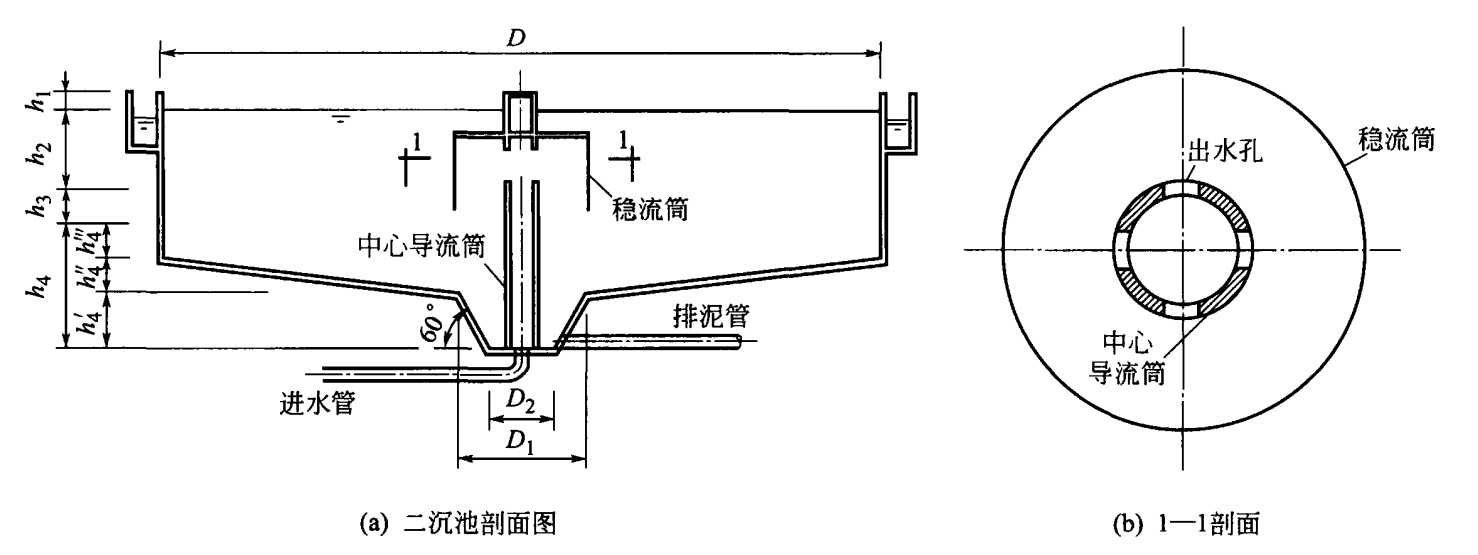
\includegraphics[width=\textwidth]{figures/Sketch of an ordinary radial type secondary sedimentation tank.png}
	\caption{普通辐流式二沉池计算草图\cite[p.225]{《城市污水厂处理设施设计计算(第三版)》}}
	\label{fig:Sketch of an ordinary radial type secondary sedimentation tank}
\end{figure}

\begin{enumerate}
	\item 沉淀部分水面面积 $F$
	
	根据生物处理段的特性,选取二沉池表面负荷 $q=0.7$ m$^3$/(m$^2\cdot$h)\footnote{普通辐流式沉淀池表面负荷一般不大于 2.5 m$^3$/(m$^2\cdot$h)。\cite{《城市污水厂处理设施设计计算(第三版)》}},设两座沉淀池即 $n=2$,则
	\begin{equation}
		F=\dfrac{Q_{max}}{nq} = \dfrac{58100}{2\times 0.7\times 24} \;\text{m$^2$} = \eval{\dfrac{58100}{2\times 0.7\times 24}}[2] \;\text{m$^2$}
	\end{equation}

	\item 池子直径 $D$
	
	\begin{align}
		D=\sqrt{\dfrac{4F}{\pi}} &= \sqrt{\dfrac{4\times 1729.17}{\pi}} \;\text{m} = \eval{\sqrt{\dfrac{4\times 1729.17}{\pi}}} \;\text{m} \\
		& \approx 47 \;\text{m(向上取整)} \notag
	\end{align}

	\item 校核固体负荷 $G$
	
	\begin{align}
		G = \dfrac{24(1+R)Q_0X}{F} & = \dfrac{24\times(1+100\%)\times 58100 \times 4}{1729.17 \times 2\times 24} \quad\text{kg/(m$^2\cdot$d)}  \\
		&= \eval{\dfrac{24\times(1+1)\times 58100 \times 4}{1729.17 \times 2\times 24}}[3] \quad\text{kg/(m$^2\cdot$d)} \notag \\
		% & \in [140,160] \quad\text{kg/(m$^2\cdot$d)(符合要求)}  \notag
		& \leqslant 150 \quad\text{kg/(m$^2\cdot$d)(符合要求)}  \notag
	\end{align}
	% \footnotetext{污泥固体负荷为 $140\sim 160$ kg/(m$^2\cdot$d)。\cite{《城市污水厂处理设施设计计算(第三版)》}}

	\item 沉淀部分的有效水深 $h_2$
	
	设沉淀时间 $t=3$ h,则
	\begin{equation}
		h_2=qt = 0.7 \times 3 \;\text{m} = 2.1 \;\text{m}
	\end{equation}

	\item 污泥区的容积 $V$
	
	设计采用周边传动的刮吸泥机排泥,污泥区容积按 2 h 贮泥时间确定,则
	\begin{align}
		V=\dfrac{2T(1+R)QX}{(X+X_r)\times 24} &= \dfrac{2\times 2\times (1+100\%)\times 35000\times 4000}{(4000+10000)\times 24} \;\text{m$^3$} \\
		& = \eval{\dfrac{2\times 2\times (1+1)\times 35000\times 4000}{(4000+10000)\times 24}}[2] \;\text{m$^3$} \notag
	\end{align}
	所以,每个沉淀池污泥区的容积 $V'=V/2=1666.67$ m$^3$。

	\item 污泥区高度 $h_4$
	\begin{enumerate}
		\item 污泥斗高度
		
		设池底的径向坡度为 $i = 0.05$,污泥斗底部直径 $D_2= 1.5$ m,上部直径 $D_1=3.0$ m,倾角 $\alpha=60^{\circ}$,则
		\begin{align}
			h_4' =\dfrac{D_1-D_2}{2}\cdot \tan{\alpha} = \dfrac{3.0-1.5}{2}\times \tan{60^{\circ}} \;\text{m} =\eval{\dfrac{3.0-1.5}{2}\times \tan{60/180*\pi}}[2] \;\text{m}
		\end{align}
		\begin{align}
			V_1 = \dfrac{\pi h_4'}{12}\cdot(D_1^2+D_1D_2+D_2^2) &= \dfrac{1.3 \pi}{12}\times(3.0^2+3.0\times 1.5+1.5^2) \;\text{m$^3$} \\
			&= \eval{\dfrac{\pi \times 1.3}{12}\times(3.0^2+3.0\times 1.5+1.5^2)}[2] \;\text{m$^3$} \notag
		\end{align}

		\item 圆锥体高度
		
		\begin{align}
			h_4'' =\dfrac{D-D_1}{2}\cdot i = \dfrac{47-3}{2}\times 0.05 \;\text{m} =\eval{\dfrac{47-3}{2}\times 0.05}[2] \;\text{m}
		\end{align}
		\begin{align}
			V_2 = \dfrac{\pi h_4''}{12}\cdot(D^2+DD_1+D_1^2) &= \dfrac{1.1 \pi}{12}\times(47^2+47\times 3.0+3.0^2) \;\text{m$^3$} \\
			&= \eval{\dfrac{\pi \times 1.1}{12}\times(47^2+47\times 3.0+3.0^2)}[2] \;\text{m$^3$} \notag
		\end{align}

		\item 竖直段污泥部分的高度
		
		\begin{align}
			h_4''' =\dfrac{V'-V_1-V_2}{F} = \dfrac{1666.67-5.36-679.34}{1729.17} \;\text{m} =\eval{\dfrac{1666.67-5.36-679.34}{1729.17}}[1] \;\text{m}
		\end{align}
		则污泥区的高度 $h$ 为
		\begin{align}
			h_4=h_4'+h_4''+h_4''' = 1.3+1.1+0.6 \;\text{m} =3.0 \;\text{m}
		\end{align}
	\end{enumerate}

	\item 沉淀池的总高度 $H$
	
	设超高 $h_1=0.3$ m,缓冲层高度 $h_3=0.5$ m,则
	\begin{align}
		H=h_1+h_2+h_3+h_4 = 0.3+2.1+0.5+3.0 \;\text{m} =\eval{0.3+2.1+0.5+3.0} \;\text{m}
	\end{align}
\end{enumerate}


\subsubsection{中心进水导流筒及稳流筒}
\begin{enumerate}
	\item 中心进水导流筒
	
	进水 $D_0=800$ mm,进水管流速 $v_0$ 为
	\begin{align}
		v_0 = \dfrac{4(1+R)Q_{max}}{n\pi D_0^2} = \dfrac{4\times(1+100\%)\times 58100}{2\pi \cdot 0.8^2 \times 86400} \;\text{m/s} =\eval{\dfrac{4\times(1+1)\times 58100}{2\pi \times 0.8^2 \times 86400}}[2] \;\text{m/s}
	\end{align}
	中心进水导流筒内流速取 $v_1=0.6$ m/s\footnote{中心进水导流筒内流速可达 1 m/s。},导流筒直径 $D_3$ 为
	\begin{align}
		D_3 = \sqrt{\dfrac{4(1+R)Q_{max}}{n\pi v_1}} &= \sqrt{\dfrac{4\times(1+100\%)\times 58100}{2\pi \cdot 0.6 \times 86400}}  \;\text{m} =\eval{\sqrt{\dfrac{4\times(1+1)\times 58100}{2\pi \cdot 0.6 \times 86400}}} \;\text{m} \\
		& \approx 1.20 \;\text{m(向上取整)}
	\end{align}
	中心进水导流筒设4个出水孔,出水孔尺寸 $B\times H=0.8 \;\text{m}\times 1.2 \;\text{m}$,出水孔流速 $v_2$ 为
	\begin{align}
		v_2 = \dfrac{(1+R)Q_{max}}{4nBH} &= \dfrac{(1+100\%)\times 58100}{4\times 2 \times 0.8 \times 1.2 \times 86400} \;\text{m/s} \\
		&=\eval{\dfrac{(1+1)\times 58100}{4\times 2 \times 0.8 \times 1.2 \times 86400}}[3] \;\text{m/s} \leqslant 0.2 \;\text{m/s} \notag
	\end{align}

	\item 稳流筒
	
	稳流筒用于稳定由中心筒流出的水流,防止对沉淀产生不利影响。稳流筒下缘淹没深度为水深的 $30\%\sim 70\%$,且低于中心导流筒出水孔下缘 0.3 m 以上。稳流筒内下降流速 $v_3$ 按最高时流量设计时一般控制在 $0.02\sim 0.03$ m/s之间,取 $v_3=0.03$,稳流筒内水流面积 $f$ 为
	\begin{equation}
		f=\dfrac{(1+R)Q_{max}}{nv_3} = \dfrac{(1+100\%)\times 58100}{2\times 0.03\times 86400} \;\text{m$^2$} = \eval{\dfrac{(1+1)\times 58100}{2\times 0.03\times 86400}}[2] \;\text{m$^2$}
	\end{equation}
	所以,稳流筒直径 $D_4$ 为
	\begin{align}
		D_4 = \sqrt{\dfrac{4f}{\pi}+D_3^2} &= \sqrt{\dfrac{4\times 22.42}{\pi}+1.2^2} \;\text{m} = \eval{\sqrt{\dfrac{4\times 22.42}{\pi}+1.2^2}} \;\text{m} \\
		& \approx 5.5 \;\text{m(向上保留一位小数)} \notag
	\end{align}

	\item 验算二沉池表面负荷
	
	二沉池有效沉淀区面积 $A$ 为
	\begin{align}
		A = \dfrac{\pi (D^2-D_4^2)}{4} = \dfrac{\pi (47^2-5.5^2)}{4} \;\text{m$^2$} = \eval{\dfrac{\pi (47^2-5.5^2)}{4}}[2] \;\text{m$^2$}
	\end{align}
	则二沉池实际表面负荷 $q'$ 为
	\begin{align}
		q' = \dfrac{Q_{max}}{nA} = \dfrac{58100}{2 \times 1711.19\times 24} \;\text{m$^3$/(m$^2\cdot$h)} = \eval{\dfrac{58100}{2 \times 1711.19\times 24}}[3]  \;\text{m$^3$/(m$^2\cdot$h)}
	\end{align}

	\item 验算二沉池固体负荷
	
	\begin{align}
		G' = \dfrac{(1+R)XQ_{max}}{1000nA} &= \dfrac{(1+100\%)\times 4000 \times 58100}{1000\times 2 \times 1711.19} \;\text{kg/(m$^2\cdot$d)} \\
		&= \eval{\dfrac{(1+1)\times 4000 \times 58100}{1000\times 2 \times 1711.19}}[2] \;\text{kg/(m$^2\cdot$d)} \notag
	\end{align}
\end{enumerate}



